\documentclass[12pt,a4paper]{article}

\usepackage[utf8]{inputenc}
\usepackage[T2A]{fontenc}
\usepackage[russian]{babel}
\usepackage{hyperref}
\usepackage[footnotes,oglav,spisok,boldsect,eqwhole,kursrab,remarks,hyperprint]{project}
\usepackage{graphicx}
\usepackage{float}
\graphicspath{{img/}}
\DeclareGraphicsExtensions{.pdf,.png,.jpg}

\begin{document}
\cover{Численные методы решения задач математической физики}{Изгиб стержня}{студент группы ФН2-71Б}{Голубенко К. М.}{к.ф-м.н. доцент кафедры ФН-2}{Родин А.С.}{}{}{2021}
\tableofcontents
\newpage
\section{Введение}
На неподвижном основании горизонтально установлен упругий стержень. Один конец стержня защемлен, другой свободен. К свободному концу
центрально приложена сжимающая сила $P$. Известны длина стержня $l$, модуль Юнга $E$. Силой тяжести в данной работе принебрегаем.

\newpage

\section{Статический случай}	
Рассмотрим стержень в простейшем одномерном случае.
\begin{figure}[H]
    \center{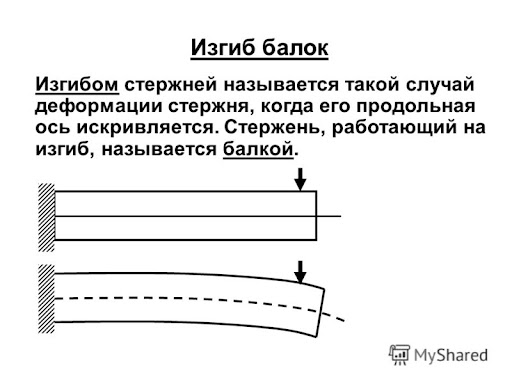
\includegraphics[scale=0.5]{1.jpg}}
    \caption{Одномерный случай}
    \label{fig:image}
\end{figure}


Пусть $u(x)$ - отклонение стержня от оси $Ox$. Тогда уравнение равновесия будет иметь следующий вид:
\begin{equation}
    \dfrac{\partial\sigma}{\partial x} = 0, 
    u(0) = 0, 
    u(l) = u_{l}.
\end{equation}
где $\sigma$ --- внутреннее напряжение. 
Воспользуемся законом Гука: $\sigma = E \varepsilon = E \dfrac{\partial u}{\partial x}$ и получим систему:
\begin{equation}
     \begin{cases}
       E \dfrac{\partial^2\sigma}{\partial x^2} = 0, \\
       u(0) = 0, & u(l) = u_{l}.
     \end{cases}
\end{equation}
Воспользуемся методом дискретизации Галеркина. Получим:
\begin{equation}
    E \int\limits_0^l \dfrac{\partial^2\sigma}{\partial x^2} N_i dx = 0,
\end{equation}
где $N_i$ - базисные функции вида:
\begin{figure}[H]
    \center{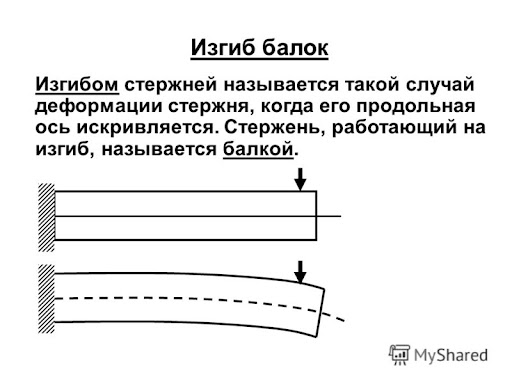
\includegraphics[scale=0.5]{1.jpg}}
    \caption{Одномерный случай}
    \label{fig:image}
\end{figure}

Преобразуем:
\begin{equation}
\label{eq1}
\begin{array}{r}
    E \int\limits_0^l \dfrac{\partial^2\sigma}{\partial x^2} N_i dx =
    E \int\limits_0^l\Big(\dfrac{\partial}{\partial x}\big( \dfrac{\partial u}{\partial x}N_i \big) -
    \dfrac{\partial u}{\partial x}\dfrac{\partial N_i}{\partial x}\Big) dx =
    E \int\limits_0^l\Big(\dfrac{\partial}{\partial x}\big( \dfrac{\partial u}{\partial x}N_i \big)\Big) dx -\\
    - E \int\limits_0^l\Big(\dfrac{\partial u}{\partial x}\dfrac{\partial N_i}{\partial x}\Big) dx = 0, 
\end{array}
\end{equation}
где $E \int\limits_0^l\Big(\dfrac{\partial}{\partial x}\big( \dfrac{\partial u}{\partial x}N_i \big)\Big) dx = 0$.

Заменим точное решение $u(x)$ на приближенное $\hat{u}$:
\begin{equation}
    u \approx \hat{u} = \sum\limits_{j = 0}^n u_j N_j.
\end{equation}

Подставим полученное выражение в \ref{eq1}:
\begin{equation}
    - E u_{i-1}\int\limits_{x_{i - 1}}^{x_i}\Big(\dfrac{\partial N_{i-1}}{\partial x}\dfrac{\partial N_i}{\partial x}\Big) dx - 
    E u_{i}\int\limits_{x_{i - 1}}^{x_{i + 1}}\Big(\dfrac{\partial N_{i}}{\partial x}\dfrac{\partial N_i}{\partial x}\Big) dx -
    E u_{i + 1}\int\limits_{x_{i}}^{x_{i + 1}}\Big(\dfrac{\partial N_{i + 1}}{\partial x}\dfrac{\partial N_i}{\partial x}\Big) dx = 0,
\end{equation}
где $i = \overline{1, n-2}.$

Найдем значения коэффициентов уравнений:
\begin{equation}
    \label{eq2}
    \begin{array}{l}
        \int\limits_{x_{i - 1}}^{x_i}\Big(\dfrac{\partial N_{i-1}}{\partial x}\dfrac{\partial N_i}{\partial x}\Big) dx = 
        \int\limits_{x_{i - 1}}^{x_{i + 1}}\Big(\dfrac{1}{x_{i-1} - x_i}\dfrac{1}{x_i - x_{i-1}}\Big) dx = -\dfrac{1}{h} = a_i, \\ \\
        \int\limits_{x_{i - 1}}^{x_{i + 1}}\Big(\dfrac{\partial N_{i}}{\partial x}\Big)^2 dx = 
        \int\limits_{x_{i - 1}}^{x_{i}}\Big(\dfrac{1}{x_i - x_{i-1}}\Big)^2 dx + 
        \int\limits_{x_{i}}^{x_{i + 1}}\Big(\dfrac{1}{x_i - x_{i+1}}\Big)^2 dx = \dfrac{2}{h} = b_i, \\ \\ 
        \int\limits_{x_{i}}^{x_{i + 1}}\Big(\dfrac{\partial N_{i+1}}{\partial x}\dfrac{\partial N_i}{\partial x}\Big) dx = 
        \int\limits_{x_{i}}^{x_{i + 1}}\Big(\dfrac{1}{x_{i+1} - x_i}\dfrac{1}{x_i - x_{i+1}}\Big) dx = -\dfrac{1}{h} = c_i.
    \end{array}
\end{equation}

Получим систему уравнений с трехдиагональной матрицей:
\begin{equation}
    \begin{cases}
      u_{i-1} a_i - u_i b_i + u_{i+1} c_i = 0, \quad i = \overline{1, n-2}\\
      u(0) = 0, \quad u(l) = u_{l}.
    \end{cases}
\end{equation}

Запишем систему в матричном виде:
\begin{equation}
    \left(
    \begin{array}{cccccc}
    -b_1 & c_1 & 0 & 0 & \ldots &  0\\
    a_{2} & -b_{2} & c_2 & 0 & \ldots &  0\\
    \vdots & \vdots & \vdots & \vdots & \ddots & \vdots\\
    0 & \ldots & a_{n-1} & -b_{n-1} & c_{n-1} & 0 \\
    0 & 0 & \ldots & a_{n-2} & -b_{n-2} & c_{n-2}
    \end{array}
    \right)
    \left(
        \begin{array}{c}
        u_1\\
        u_2\\
        \vdots\\
        u_{n-2} \\
        u_{n-1}
        \end{array}
    \right) =     \left(
        \begin{array}{c}
        0\\
        0\\
        \vdots\\
        0\\
        -u_l c_{n-1}
        \end{array}
    \right)
    \end{equation}

Решим полученную систему методом прогонкdи.f
\section{Заключение}

\begin{thebibliography}{9}
\bibitem{source1} бебебе с бабаба

\end{thebibliography}




 

\end{document} 